% SPDX-License-Identifier: CC-BY-4.0
%
% Copyright (c) 2024 Nelson Vieira and Mary Barreto
%
% @author Nelson Vieira <2080511@student.uma.pt>
% @contributor Mary Barreto <mary.barreto@staff.uma.pt>
% @license CC-BY-4.0 <https://creativecommons.org/licenses/by/4.0/legalcode.txt>
\documentclass[xcolor={svgnames},compress,aspectratio=169]{beamer}
\usetheme{Berlin}
\usecolortheme{dolphin}

\setbeamercolor*{structure}{bg=Azure,fg=MidnightBlue!50!black}

\setbeamercolor*{palette primary}{use=structure,fg=structure.bg,bg=structure.fg}
\setbeamercolor*{palette secondary}{use=structure,fg=structure.fg,bg=structure.bg}
\setbeamercolor*{palette tertiary}{use=structure,fg=structure.fg,bg=GhostWhite}
\setbeamercolor*{palette quaternary}{fg=white,bg=black}

\setbeamercolor{section in head/foot}{parent=palette primary} % Outer section of header/footer
\setbeamercolor{subsection in head/foot}{parent=palette secondary} % Inner section of header/footer

\setbeamercolor{titlelike}{parent=palette tertiary} % Main titles
\setbeamercolor{frametitle}{parent=palette tertiary,bg=GhostWhite!50}

\setbeamercolor{section in toc}{fg=darkgray,bg=Azure} % Table of contents sections
\setbeamercolor{subsection in toc}{fg=darkgray,bg=Azure} % Table of contents subsections
% \setbeamercolor{alerted text}{use=structure,fg=structure.fg!50!black!80!black}

% \setbeamertemplate{navigation symbols}{} % Hides navigation buttons at the bottom
% \setbeamertemplate{headline}{} % Hides navigation bar at the top

\setbeamercovered{transparent}

\setbeamertemplate{caption}[numbered]

% \usepackage{pgfpages}
% \pgfpagesuselayout{4 on 1}[a4paper,border shrink=5mm]

\usepackage[utf8]{inputenc}
\usepackage{adjustbox}
\usepackage{xcolor,colortbl}
\usepackage[all]{xy}
\usepackage{tikz}
\usetikzlibrary{mindmap,backgrounds}
\usepackage{graphicx}
\usepackage{multicol}
% Advanced table functions
\usepackage{tabularx,ragged2e}
\usepackage{booktabs}
% Listings extension
\usepackage{listings}
\usepackage{transparent}
\usepackage{amsmath,amssymb,amsfonts}
\usepackage[font=tiny]{caption}
\usepackage[font=tiny]{subcaption}
\usepackage{pgfplots}
\usepackage{pgf-pie}
\usepackage{tcolorbox}
\usepackage{svg}
\setsvg{inkscape = "C:/Program Files/Inkscape/bin/inkscape.exe"}
\svgsetup{inkscapepath=svgsubdir}
\def\myversion{0.5}

\title[Privacy and Digital Literacy in the Internet of Things]{{\normalsize 22nd International Conference e-Society 2024} \\ Privacy and Digital Literacy in the Internet of Things}
% \subtitle{}
\author{\href{mailto:2080511@student.uma.pt}{Nelson Vieira} and \href{mailto:mary.barreto@staff.uma.pt}{Mary Barreto}}
\institute[\href{https://www.uma.pt/}{University of Madeira}]{University of Madeira\\Faculty of Exact Sciences and Engineering}
\date{{\scriptsize Last Update: \today}}

\setbeameroption{hide notes}

\makeatletter
    \newenvironment{withoutheadline}{
        \setbeamertemplate{headline}[default]
        \def\beamer@entrycode{\vspace*{-\headheight}}
    }{}
\makeatother

\begin{document}

\begin{withoutheadline}
    \begin{frame}
        % \centering\includegraphics[width=90pt]{assets/images/uma_logo.png}
        \maketitle
    \end{frame}
\end{withoutheadline}

\begin{frame}{Table of Contents}
    % Use hideallsubsections for longer presentations
    % \tableofcontents[hideallsubsections]
    \begin{multicols}{2}
        \tableofcontents
    \end{multicols}
\end{frame}

\section{Introduction}

% Option [fragile] needed for lstlisting
\begin{frame}[fragile]
    \begin{multicols}{2}
        \centering
        {\footnotesize What is privacy?}
        \begin{figure}
            \centering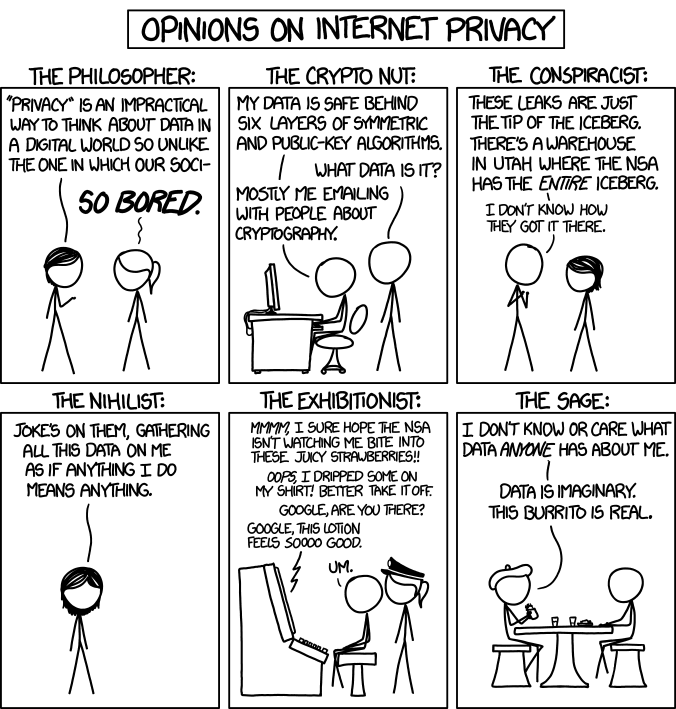
\includegraphics[width=155pt]{assets/images/privacy_opinions.png}\\
            \textcolor{gray}{{\tiny \textcopyright \href{https://xkcd.com/1269/}{Randall Munroe}, \href{https://creativecommons.org/licenses/by-nc/2.5/}{CC BY-NC 2.5 License}}}
        \end{figure}

        \columnbreak
        \vspace*{\fill}
\begin{lstlisting}[language=sh,escapechar=\%]
    diff privacy.c
    %\big\uparrow%     %\textcolor{blue}{@@ -1,1 +1,1 @@}%
    1 %\textcolor{red}{- Privacy}%
    1 %\textcolor{green!60!black!80}{+ Security}%
    %\big\downarrow%     ...
\end{lstlisting}
        \vspace*{\fill}
    \end{multicols}
\end{frame}

\note{
    There is some contention on the definition of privacy. Most literature assumes
    that privacy is equal to security or that it is only a part of it, as such
    by creating better security systems they assume to alse solve privacy problems.
    This work takes privacy on its own and goes out looking for challenges and solutions
    to solve privacy issues on IoT systems.
}

\begin{frame}{Introduction}
    The advent of ubiquitous computing has resulted in the widespread use of
    Internet of Things devices. These devices open up
    new avenues for the collection and exploitation of user and non-user personal
    data. Most end users are not even aware or have little control over the
    information that is being collected about them by these systems.

    This work took a rounded approach to this problem by doing:
    \begin{itemize}
        \item<1-> Literature review;
        \item<2-> A survey.
    \end{itemize}
\end{frame}

\note{
    This work tackles privacy literacy in IoT systems. An holistic approach was taken
    and consisted in doing a systematic literature review, a survey and a mobile application.
}

\section{Methodology}

\subsection{Survey}

\begin{frame}[shrink]{Survey}
    \begin{multicols}{2}
        86 Questions
        \begin{itemize}
            \item General knowledge and attitudes towards privacy
            \item Disposition for sharing personal information
            \item Privacy concerns
            \item Current online habits and practices
            \item Profile identification
            \item Knowledge and habits regarding the Internet of Things
            \item Demographic data
        \end{itemize}

        \columnbreak
        \vspace*{\fill}
        \begin{figure}
            \centering
            
\includegraphics[width=45pt]{assets/images/forms.png}
            % \caption{Google Forms}
        \end{figure}
        \vspace*{\fill}
    \end{multicols}
\end{frame}

\note{
    Survey with varied questions from general privacy concerns to online habits and IoT literacy.
    86 questions under 7 main topics of interest from privacy attitudes, concerns, online habits to IoT knowledge and usage.
}

\section{Conclusion and Future Work}

\subsection{Future Work}

\begin{frame}{Future Work}
    Improvements for survey
    \begin{itemize}
        \item[$\bullet$]
        More lean survey;
        \item[$\bullet$]
        Some kind of reward for participants;
    \end{itemize}
    Topics for further research
    \begin{itemize}
        \item[$\bullet$]
        Privacy literacy in IoT systems;
        \item[$\bullet$]
        Application of privacy in the design/development of IoT systems;
        \item[$\bullet$]
        User-centric approaches to IoT privacy.
    \end{itemize}
\end{frame}

\note{
    Some notes here.
}

\subsection{Conclusion}

\begin{frame}{Conclusion}
    \begin{itemize}
        \item[$\bullet$]
        Standalone IoT privacy literature review;
        \item[$\bullet$]
        Tests from majority viewpoint of portuguese users;
        \item[$\bullet$]
        User testing reveals there is a large privacy knowledge gap;
    \end{itemize}
\end{frame}

\note{
    This work contributed to the overall body of research by compiling and reviewing
    other works with the perspective of privacy as a distinct subject matter rather than
    an extension of security, as many publications imply. The survey conducted
    on the perception of individuals on privacy in IoT systems portrays the majority
    viewpoint of portuguese people, since 60\% of participants were portuguese.
}

\begin{frame}
    \begin{center}
        {\large Thank you for your attention.}
    \end{center}
\end{frame}

\section*{References}

\begin{frame}[allowframebreaks]{References}
    \bibliographystyle{IEEEtran}
    {\footnotesize \bibliography{assets/references}}
\end{frame}

\end{document}
